\documentclass[a4paper,10pt,oneside]{scrbook}

\usepackage[utf8x]{inputenc}
%\usepackage{polski}
\usepackage{fancyvrb}
\usepackage{graphicx}
\usepackage[bottom=10em]{geometry}
\usepackage{color}
\usepackage{xcolor}
\usepackage{listings}

\lstset{literate={ą}{{\k{a}}}1 {ć}{{\'c}}1 {ł}{{\l{}}}1 {ń}{{\'n}}1 {ę}{{\k{e}}}1 {ś}{{\'s}}1 {ż}{{\.z}}1 {ó}{{\'o}}1 {ź}{{\'z}}1 {Ą}{{\k{A}}}1 {Ć}{{\'C}}1 {Ł}{{\L{}}}1 {Ń}{{\'N}}1 {Ę}{{\k{E}}}1 {Ś}{{\'S}}1 {Ż}{{\.Z}}1 {Ó}{{\'O}}1 {Ź}{{\'Z}}1 }

\lstset{language=Java,captionpos=t,tabsize=3,frame=single,keywordstyle=\color{blue},
        commentstyle=\color{gray},stringstyle=\color{red},numbers=left,numberstyle=\tiny,
        numbersep=5pt,breaklines=true,showstringspaces=false,basicstyle=\footnotesize,emph={label}}

\title{User manual \\ Inforex \\ {\large version 0.1}}
\author{Michał Marcińczuk}

\begin{document}

\maketitle

%##############################################################################
\chapter{Introduction}
%------------------------------------------------------------------------------
\section{About Inforex}
%------------------------------------------------------------------------------


Inforex can be accessed from any standard-compliant web browser supporting JavaScript. The user interface has a form of dynamic HTML pages using the AJAX technology. The server part of the system is written in PHP and the data is stored in MySQL database. The system make use of some external tools that are installed on the server or can be accessed via web services.

The documents are stored in the database in the original format --- either plain text, XML or HTML. Tokenization and sentence segmentation is optional and is stored in a separate table. Tokens are stored as pairs of values representing indexes of first and last character of the tokens and sets of features representing the morpho-syntactic information. Annotations\footnote{Annotation is understood as a label attached to a continuous piece of text. Additional information can be attached to the annotation as a pair of strings: \{argument; value\}.} created by user are stored in the same way as tokens (pair of character indexes) but in additional table. Character indexes omit all the white spaces and XML/HTML tags. In addition, HTML entities are counted as one character. 

%------------------------------------------------------------------------------
\section{License}
%------------------------------------------------------------------------------

Inforex is published under GNU General Public License v3.0 (GPL).


%##############################################################################
\chapter{System administration}
%------------------------------------------------------------------------------

%This section contains actions which can be performed by Inforex administrators.

%------------------------------------------------------------------------------
\section{Users}
%------------------------------------------------------------------------------


%------------------------------------------------------------------------------
\section{Annotation schema}
%------------------------------------------------------------------------------

  This section covers what is annoation schema and how to edit it.

  Annotation is a label which can be attached to any text fragment in a document. A hierarchy of annotation categories is called an annotation schema. Inforex supports two-level hierarchy schema. Annotation schema is defined at the system level and the annotation sets can be shared between different corpora.

  Modification of annotation schema requires \verb|admin| role. To modify the annotation schema go to \verb|Administration| \verb|> Annotations| page. The page is divided into three panels (see Figure~\ref{fig:inforex-administration-annotatons}):
\begin{enumerate}
 \item \textbf{Select set} --- list of all sets of annotations. Allows to create new schemas and change name of existing one (the edit and delete options are available after selecting a row in the table).
 
 \item \textbf{Edit annotation subsets and categories} --- allows to modify the annotation subsets and categories. The panel contains two boxes:

 \begin{itemize}
    \item \textbf{Subsets} --- available after choosing a annotation schema from the previous box. It contains a list of annotation subsets grouping annotation categories (types).
    
    \item \textbf{Categories} --- available after choosing a subset from the previous box.
    Every annotation is described with following attributes:
    \begin{itemize}
      \item \verb|name| --- symbolic name of annotation category. It must be unique amont all annotation categories. Cannot be changed later.
      \item \verb|short| --- is optional and when provided used instead of name in the toolbox with the list of annotations {\[TODO podac\_gdzie\_wykorzystywane\_sa\_skrocone\_opisy\]},
      \item \verb|description| --- annotation category description,
      \item \verb|css| --- CSS style used to format the annotations in the document view.
    \end{itemize}
    
 \end{itemize}

  \item \textbf{Attach/detach annotation set to corpora} --- is used to defined in which corpora given set of annotation can be used. Annotations set can be also attached to corpora on the corpora setting page (see Section~\ref{sec:corpus-settings-annotations}).
 
 \end{enumerate}

 \begin{figure}[h]
    \centering
    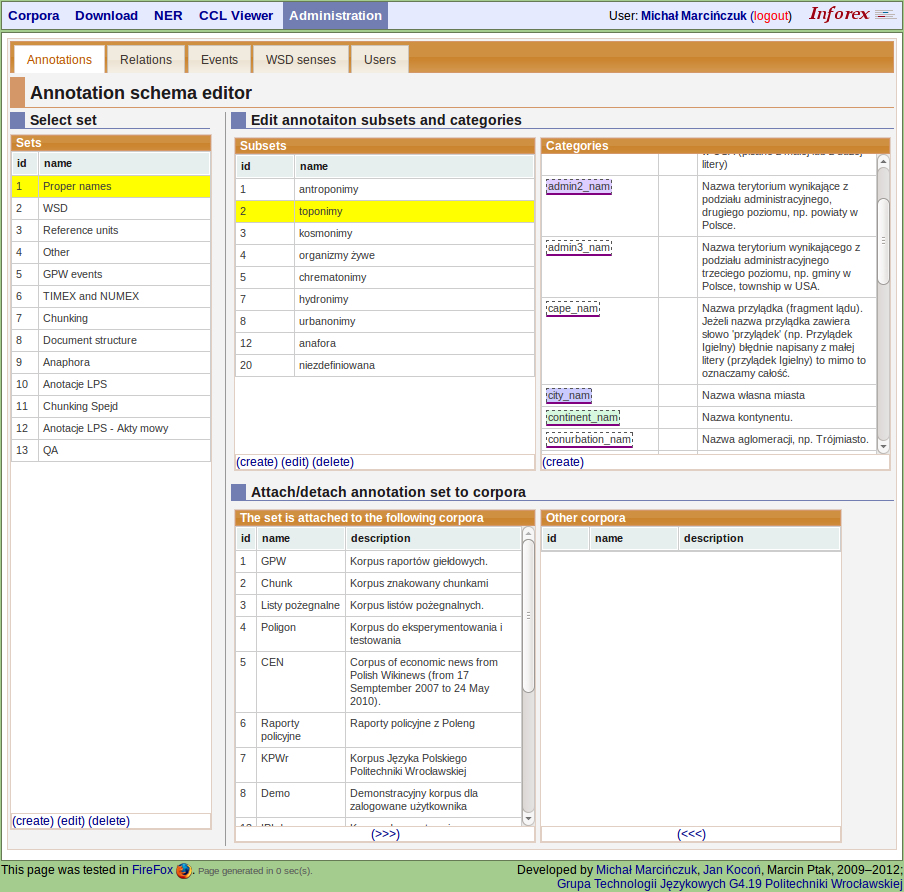
\includegraphics{images/inforex-administration-annotations.png}
    \caption{Page for annotation schema management.}
    \label{fig:inforex-administration-annotatons}
  \end{figure}


%------------------------------------------------------------------------------
\section{Relation schema}
%------------------------------------------------------------------------------

%------------------------------------------------------------------------------
\section{Event schema}
%------------------------------------------------------------------------------

%------------------------------------------------------------------------------
\section{WSD senses}
%------------------------------------------------------------------------------


%##############################################################################
\chapter{Corpus settings}
\label{sec:corpus-settings}
%------------------------------------------------------------------------------

%------------------------------------------------------------------------------
\section{Create new corpus}
%------------------------------------------------------------------------------

This option requires \verb|admin| role. To create a new corpus go to the \verb|Corpora| page and click button ``Create new corpora'' located below the table with existing corpora (see Figure~\ref{fig:inforex-start-page}). Then enter corpus name and description and press \verb|Ok|. The new corpus will have restricted access by default. The corpus settings can be change on the \verb|Settings| page (see Section~\ref{sec:corpus-settings}).

\begin{figure}[h]
\centering
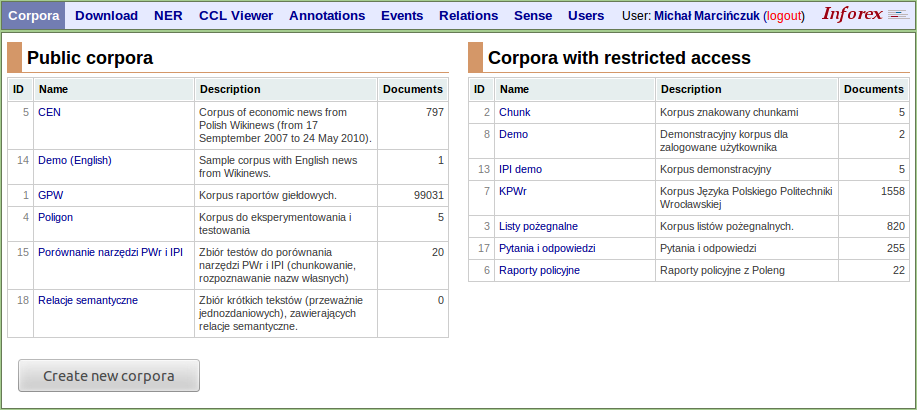
\includegraphics{images/inforex-corpora-new.png}
\caption{Inforex start page for logged in user.}
\label{fig:inforex-start-page}
\end{figure}

%------------------------------------------------------------------------------
\section{Subcorpora}
\label{sec:corpus-subcorpora}
%------------------------------------------------------------------------------

Within a corpus documents are divided into subcorpors. Before adding new document you must create at least one subcorpus. In order to create a subcorpus go to \verb|Settings|, next \verb|Subcorpora| and click \verb|create|.

%------------------------------------------------------------------------------
\section{Annotation sets}
\label{sec:corpus-settings-annotations}
%------------------------------------------------------------------------------

%------------------------------------------------------------------------------
\section{Users and permissions}
%------------------------------------------------------------------------------

%------------------------------------------------------------------------------
\section{Document perspectives}
%------------------------------------------------------------------------------

\subsection{Available perspectives}

\begin{tabular}{lcp{8cm}}
  \hline
  \multicolumn{3}{c}{Presentation} \\
  \hline
  • \textbf{Viewe}\\
  • \textbf{View Document}\\
  • \textbf{View Content}\\
  • \textbf{View Anaphora}\\
  • \textbf{Transcription}\\
  • \textbf{Topis}\\
  • \textbf{History of changes}\\
  • \textbf{TEI}\\
  • \textbf{Tokenization} \\
  \hline
  \multicolumn{3}{c}{Modification}\\
  \hline
  • \textbf{TaKIPI}\\  
  • \textbf{Edit Metadata}\\
  • \textbf{Edit Content}\\
  • \textbf{Edit Anaphora}\\
  • \textbf{Annotator} & --- & Perspective for annotation and relation modification. \\
  • \textbf{Bootstrapping}\\
  • \textbf{WSD}\\
  • \textbf{Magane images}\\
  \hline
\end{tabular}


%------------------------------------------------------------------------------
\section{Flags}
%------------------------------------------------------------------------------

%------------------------------------------------------------------------------
\section{Events}
%------------------------------------------------------------------------------

%------------------------------------------------------------------------------
\section{Metadata}
%------------------------------------------------------------------------------


%##############################################################################
\chapter{Corpus management}
%------------------------------------------------------------------------------
\section{Add new document}
%------------------------------------------------------------------------------

\subsection{GUI}
%------------------------------------------------------------------------------

New document can be added by a user with a role \verb|admin| or a corpus role \verb|add_document|. Before you add new document make sure there is at least one subcorpus (see Section~\ref{sec:corpus-subcorpora}).

\subsection{Batch upload}
%------------------------------------------------------------------------------

A batch of documents can be uploaded using the \verb|upload.php| script located in the folder \verb|local.php|.

\subsubsection{Script description}
\begin{verbatim}
 Execute: 
  php upload.php [parameters]

 Parameters: 
 -U, --db-uri <URI>             - connection URI: user:pass@host:ip/name
 -f, --folder <path>            - path to a folder with documents
 -F, --format <format>          - document format; one of: plain, xml, premorph
 -s, --subcorpus <id>           - subcorpus ID
 -u, --user <id>                - user ID
     --update                   - update files content and insert new one
     --insert                   - insert files into empty subcorpus
     --cleaned                  - mark as cleaned 
\end{verbatim}

\subsubsection{Usage examples}



%------------------------------------------------------------------------------
\section{Delete corpus}
%------------------------------------------------------------------------------


%##############################################################################
\chapter{Document management}
%------------------------------------------------------------------------------
This section contains description of actions which can be performed on documents already added to the corpus.

%------------------------------------------------------------------------------
\section{Metadata}
%------------------------------------------------------------------------------


%------------------------------------------------------------------------------
\section{Content}
%------------------------------------------------------------------------------


%------------------------------------------------------------------------------
\section{Annotation}
%------------------------------------------------------------------------------



\end{document}
